\begin{figure*}
  \centering     
     %   \begin{subfigure}[b]{0.49\textwidth}
     %   \caption{Expected}
     %     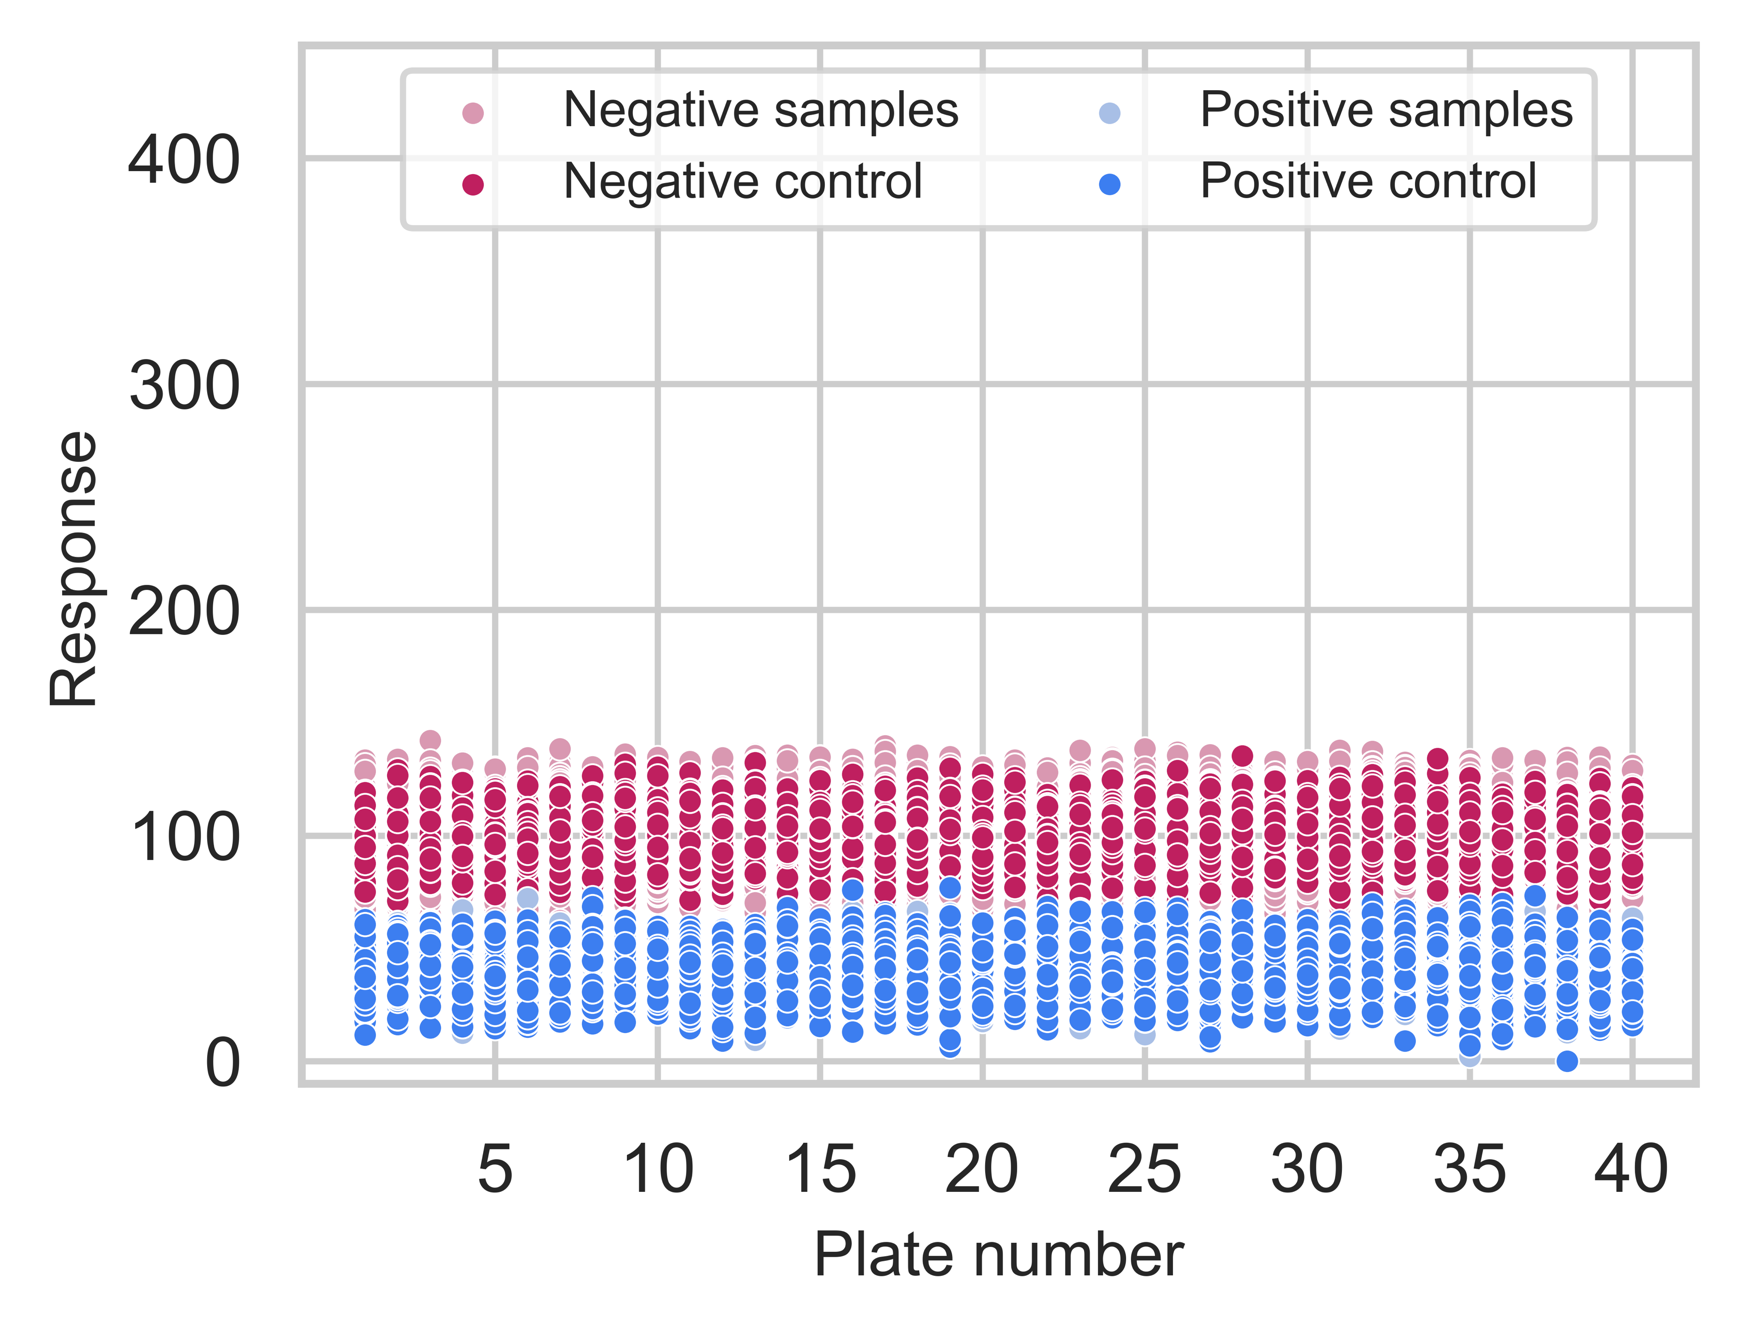
\includegraphics[width=\textwidth]{figures/screening-bowl-0.03-10-10-0.99-stdev-3-4-expected.png}
     %     \label{fig:expected}
     % \end{subfigure}
     % \hfill


       \begin{subfigure}[b]{0.31\textwidth}
         \centering
         \caption{Random}
         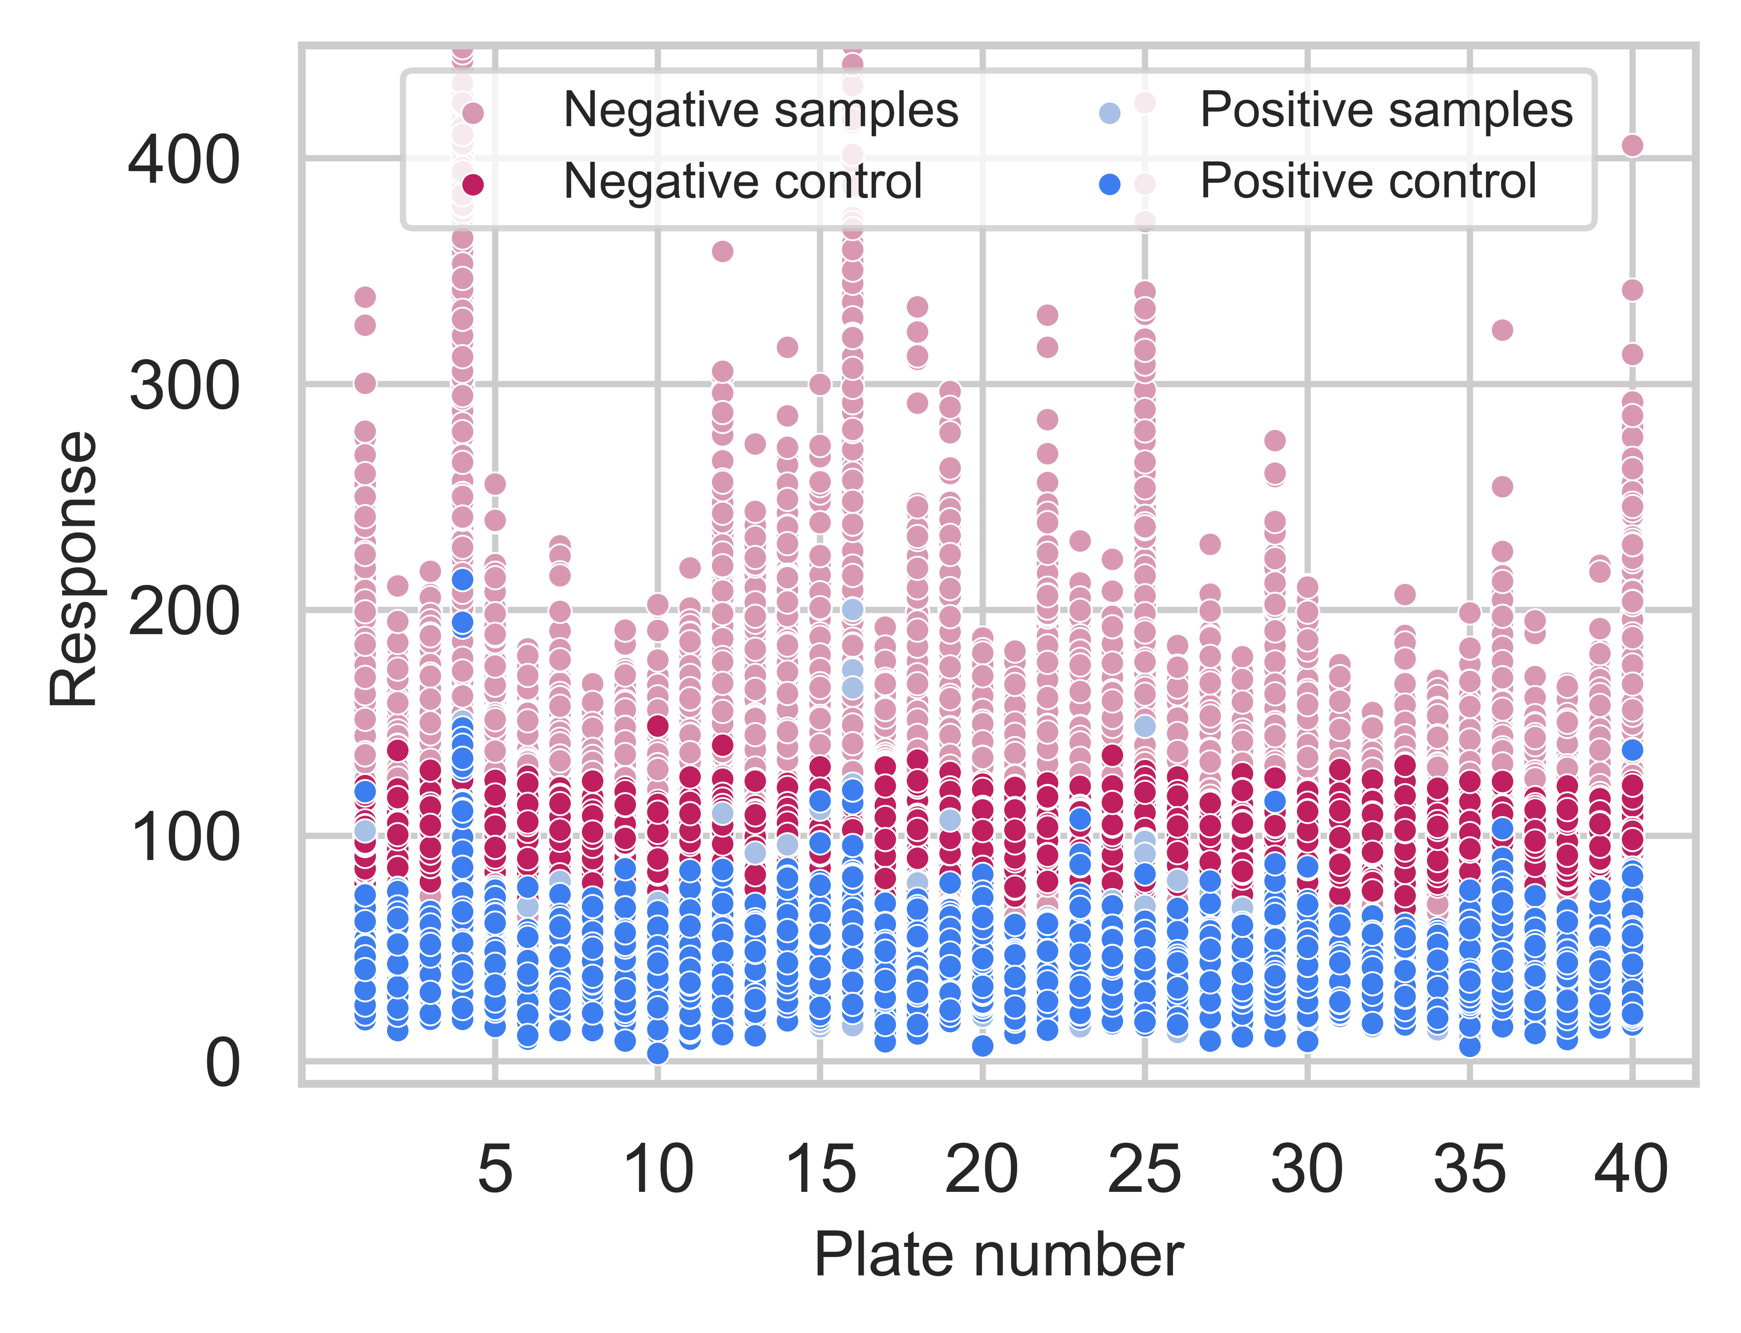
\includegraphics[width=\textwidth]{figures/screening-bowl-0.03-10-10-0.99-stdev-3-4-random.png}
         %\label{fig:random}
     \end{subfigure}
     \hfill
     \begin{subfigure}[b]{0.31\textwidth}
         \centering
         \caption{PLAID}
         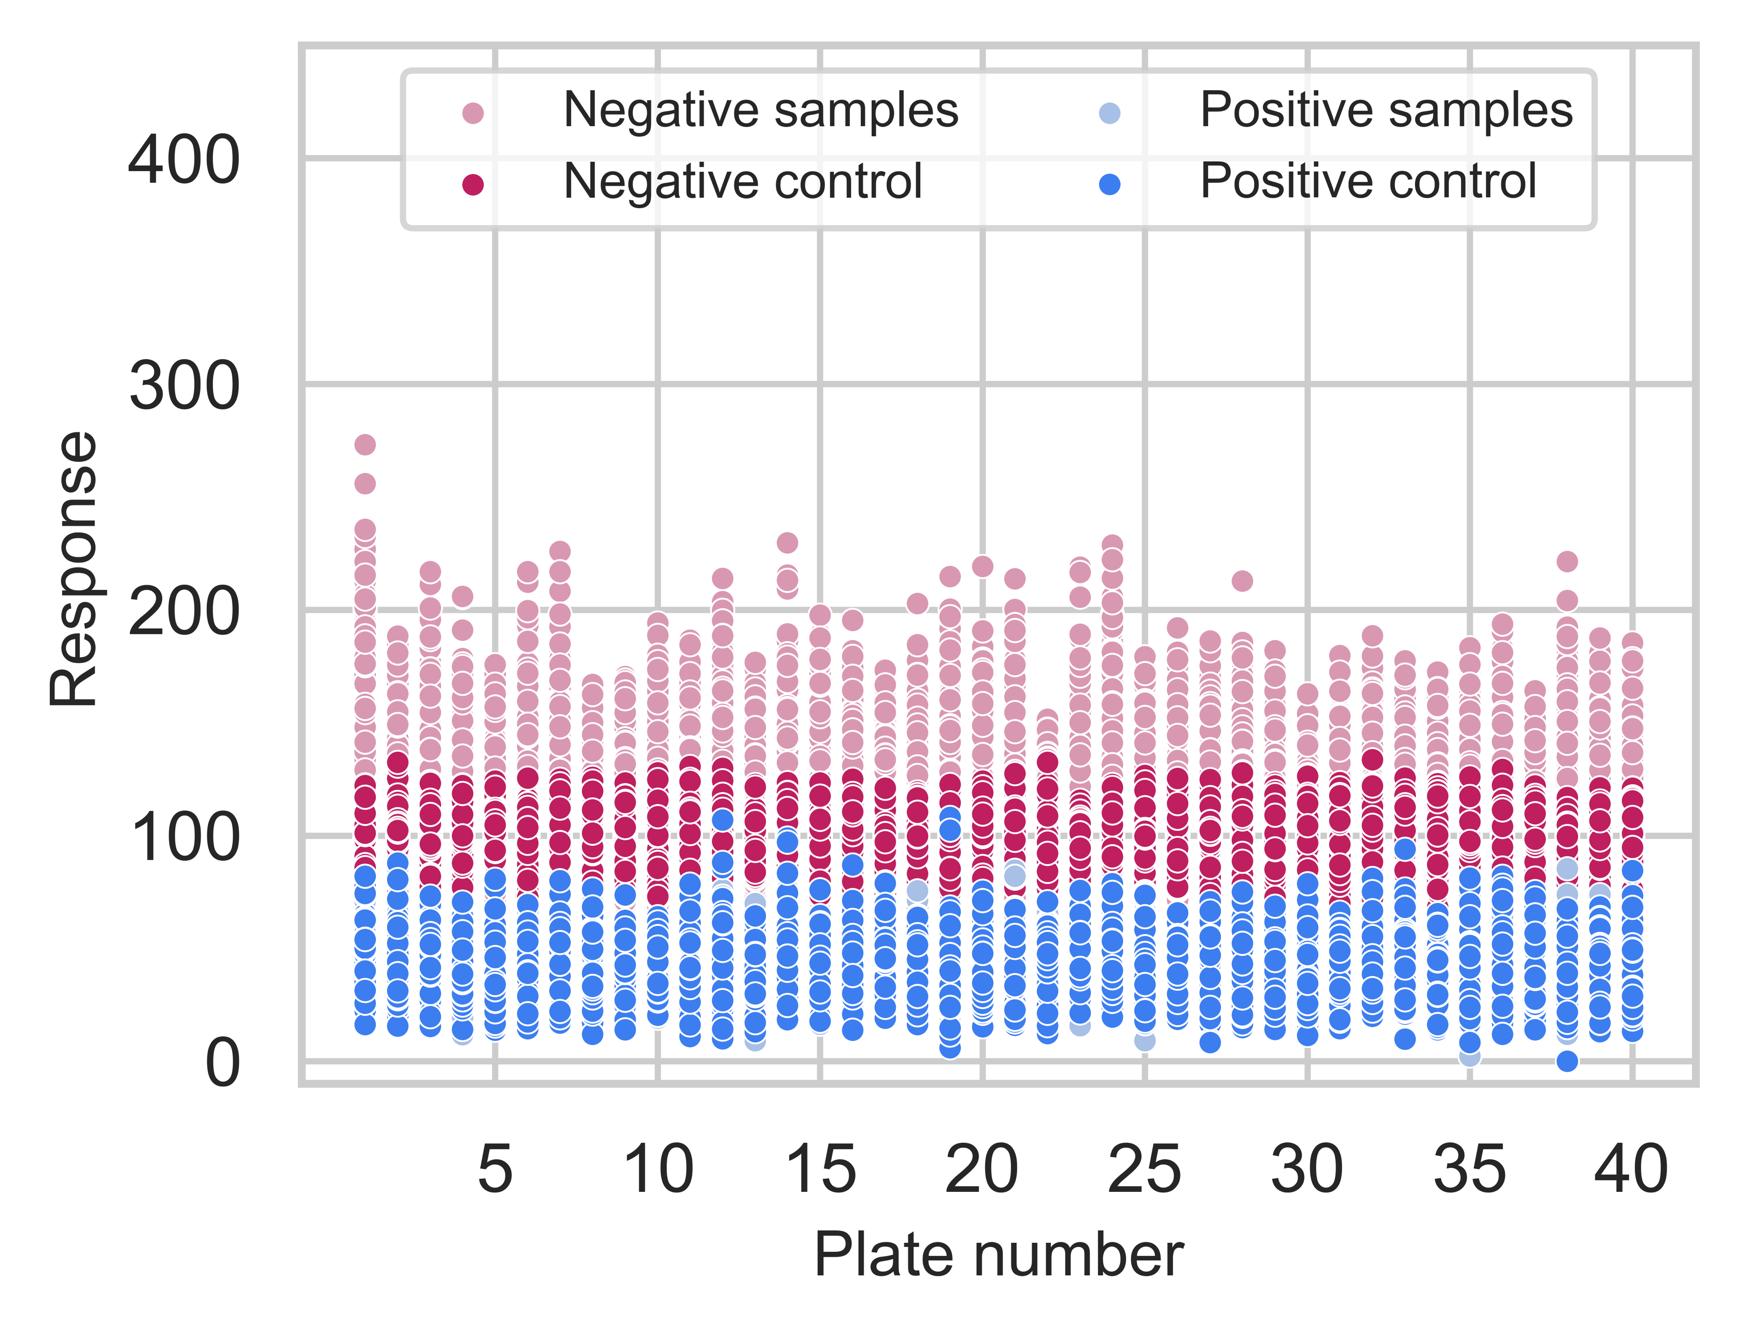
\includegraphics[width=\textwidth]{figures/screening-bowl-0.03-10-10-0.99-stdev-3-4-plaid.png}
         %\label{fig:effective}
     \end{subfigure}
     \hfill
     \begin{subfigure}[b]{0.31\textwidth}
         \centering
         \caption{COMPD}
         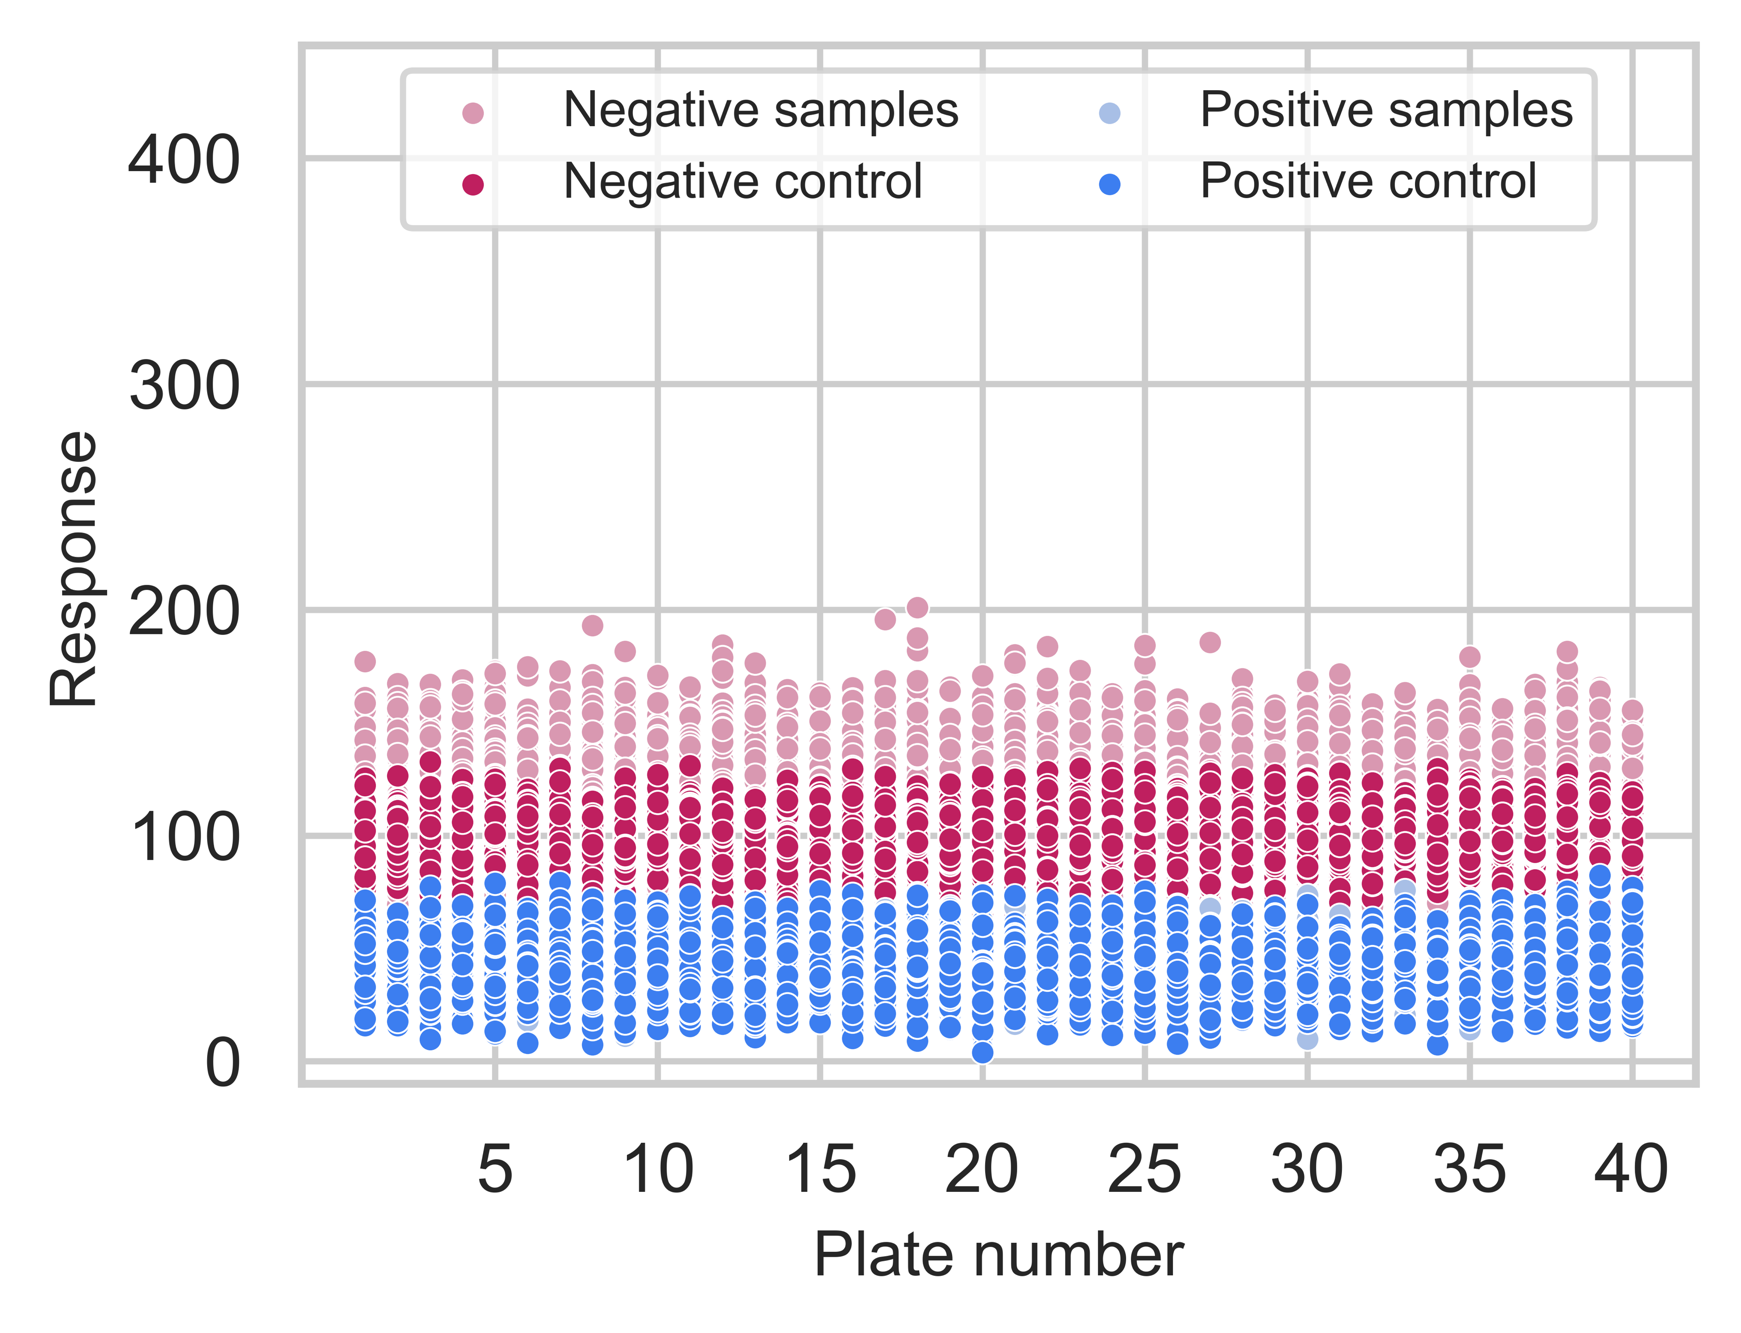
\includegraphics[width=\textwidth]{figures/screening-bowl-0.03-10-10-0.99-stdev-3-4-compd.png}
         %\label{fig:border}
     \end{subfigure}
  
     \caption{Comparison between expected and obtained values for
       screening experiments using $10$~positive and $10$~negative
       controls on 384-well plates with only 1~replicate, 1\%~hit-rate
       and mild bowl-shaped plate effects.} 
        \label{fig:screening-data-collection-mild}
\end{figure*}